\documentclass{article}
\usepackage[a4paper, margin=2.5cm]{geometry} % Mengatur margin untuk teks utama
\usepackage{tikz}
\usepackage{eso-pic}
\usepackage{xcolor}
\usepackage{graphicx}
\usepackage{lipsum} % Untuk contoh teks

% Definisikan Warna
\definecolor{colorOrange}{HTML}{F6921E} % Orange dari gambar
\definecolor{colorRed}{HTML}{E85D5D}   % Warna mirip merah muda/salmon di gambar
\definecolor{colorGrey}{HTML}{88929E}   % Warna mirip abu-abu kebiruan di gambar
\definecolor{colorHeader}{HTML}{7A748A} % Warna abu-abu header

%------------------------------------------------------------------------------------------------------------------------------------

\begin{document}

% Hanya tambahkan background ini di halaman pertama (judul)
\AddToShipoutPicture*{
    \begin{tikzpicture}[remember picture, overlay]

        % ==============================================
        % Latar Belakang - Bentuk Geometris (Kiri Bawah & Kiri Tengah)
        % ==============================================
        
        % Bentuk abu-abu besar di kiri bawah
        % Dimulai di sudut kiri bawah halaman (current page.south west)
        \fill[colorGrey, opacity=0.8] 
            ([xshift=0cm, yshift=0cm]current page.south east) 
            rectangle 
            ([xshift=12.5cm, yshift=2cm]current page.south west);

        % Bentuk oranye di tengah-kiri, sedikit di atas yang abu-abu
        \fill[colorOrange, opacity=0.7] 
            ([xshift=2cm, yshift=2cm]current page.south west) 
            rectangle 
            ([xshift=4.5cm, yshift=10cm]current page.south west);

        % Bentuk abu-abu kecil di tengah-kiri (seperti di gambar)
        \fill[colorGrey, opacity=0.8] 
            ([xshift=0cm, yshift=10.5cm]current page.south west) 
            rectangle 
            ([xshift=3.5cm, yshift=14cm]current page.south west);

        % ==============================================
        % Latar Belakang - Header (Atas)
        % ==============================================

        % Header abu-abu (Kanan)
        \fill[colorHeader] 
            (current page.north east) 
            rectangle 
            ([xshift=-0cm, yshift=-1.5cm]current page.north west);

        % Header oranye (Sudut Kanan Atas)
        \fill[colorOrange] 
            ([xshift=-5cm, yshift=-0cm]current page.north east) 
            rectangle 
            ([xshift=0cm, yshift=-1.5cm]current page.north east);
            
        % ==============================================
        % Kotak Besar untuk Foto Produk (Merah/Salmon)
        % ==============================================
        
        % Menggunakan 'current page.north east' dan 'current page.north west' untuk penempatan
        % (Menempatkan kotak besar di bagian atas tengah)
        \fill[colorGrey] 
            ([xshift=4.5cm, yshift=-3cm]current page.north west) 
            rectangle 
            ([xshift=-4.5cm, yshift=-15cm]current page.north east);
            
        % Teks di dalam Kotak Foto
        \node[text=white, font=\Large\bfseries] at ([yshift=-9cm]current page.north) {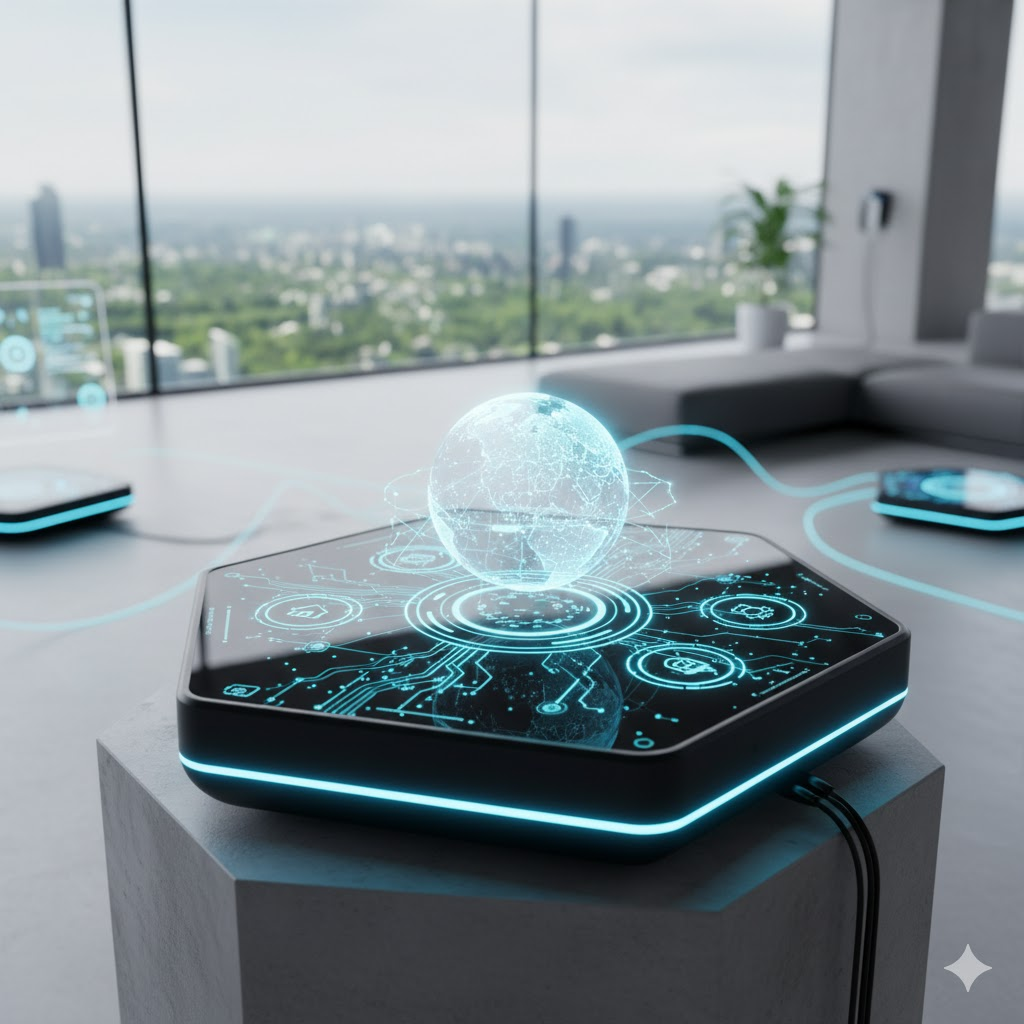
\includegraphics[height=10cm]{image/doc/contoh product.jpg}};

        % ==============================================
        % Teks Header (di atas latar belakang abu-abu)
        % ==============================================
        \node[text=white, font=\Large\bfseries] at ([yshift=-0.75cm]current page.north) 
            {CAPSTONE DESIGN DOCUMENTS};
            
            \node[text=white, font=\Large\bfseries] at ([xshift=8cm, yshift=-0.75cm]current page.north) 
            {TA2526.01.099};
    \end{tikzpicture}
}

%------------------------------------------------------------------------------------------------------------------------------------

% Teks Utama Halaman Judul (Di luar overlay TikZ)

\vspace*{13cm} % Spasi agar konten teks utama dimulai di bawah kotak foto
% Bagian Bawah
\centering
\begin{tikzpicture}[remember picture] % Menggunakan tikz untuk ikon sosial

    % Ikon Sosial Media (Menggunakan node dengan label)
    \node (social) at (0, 0) {
        
\includegraphics[height=2cm]{image/doc/prodi.png}   
\includegraphics[height=2cm]{image/doc/logo-itera.png}       
    };
    
    % Contoh Penempatan Ikon (jika menggunakan font atau simbol)
    % \node[font=\Huge] at (0, 0) {$\Psi$ \quad $\Sigma$ \quad $\Theta$ \quad $\Omega$}; 
    
    % URL
    
\end{tikzpicture}
\centering % Teks di tengah

% Nama Produk
{\Huge\bfseries Nama Product \par}
\vspace{1cm}

% Authors
{\large Authors \par}
\vspace{0.5cm}

% Deskripsi Produk (Perkiraan penempatan berdasarkan gambar)

   
{\large  Product Description \par}
\vspace{0.5cm}

% Nama Program Studi (Perkiraan penempatan berdasarkan gambar)
{\LARGE  Program Studi Teknik Elektro \\
Fakultas Teknologi Industri \\ Institut Teknologi Sumatera \\
2025

\par}
\vspace{0.5cm}
\vfill % Dorong sisa konten ke bawah



\vspace{0.5cm} % Spasi tambahan di bagian bawah

% PENTING: Anda mungkin perlu mengkompilasi dokumen DUA KALI (setelah menjalankan PdfLaTeX atau sejenisnya) agar posisi overlay (TikZ) terrender dengan benar (karena opsi 'remember picture, overlay').
\end{document}